%===============================================================================
% ifacconf.tex 2022-02-11 jpuente  
% 2022-11-11 jpuente change length of abstract
% Template for IFAC meeting papers
% Copyright (c) 2022 International Federation of Automatic Control
%===============================================================================
\documentclass{ifacconf}

\usepackage{graphicx}      % include this line if your document contains figures
\usepackage{natbib}        % required for bibliography
%===============================================================================
\begin{document}
\begin{frontmatter}

\title{GEOSPATIAL ANALYSIS FOR THE SELECTION OF ZONES UNDERGROUND STORAGE IN COLOMBIA: SINÚ-SAN JACINTO BASIN CASE } 




\author[First]{G.ARIZA, L.} 



\address[First]{Universidad Nacional de Colombia, sede Medellin (e-mail: anggarciaar@unal.edu.co).}


\begin{abstract}                % Abstract of 50--100 words

This study focuses on the Sinú-San Jacinto basin and aims to select an optimal zone for underground CO2 storage using geospatial analysis techniques. Four key factors are considered: proximity to CO2-emitting cities, presence of mud volcanoes, seismicity, and data availability including well data, 2D seismic lines, and 3D seismic data.

The integration of these factors allows for the identification of an optimal exploration zone in the Sinú-San Jacinto basin. The Luruaco Block stands out as a technically and economically viable area for underground CO2 storage, characterized by low seismicity, absence of mud bodies that pose a risk of gas escape, availability of well data, 2D seismic lines, and 3D seismic data, and proximity to major emission sources within the basin.
\end{abstract}

\begin{keyword}
Underground Storage, CO2, Sinu San Jacinto Basin, geospatial analysis.
\end{keyword}

\end{frontmatter}
%===============================================================================

\section{Introduction}
In recent years, the imperative to address climate change has necessitated intensified efforts to mitigate greenhouse gas emissions. Carbon capture and storage (CCS) has emerged as a promising strategy, involving the capture and subsurface storage of carbon dioxide (CO2) emissions from industrial processes. However, successful CCS implementation critically hinges upon the identification of optimal zones for underground CO2 storage\cite{Chen2015}.

This study focuses on the Sinú-San Jacinto basin and aims to employ geospatial analysis techniques to select a suitable exploration zone for underground CO2 storage\cite{Godec2014}. Four key factors will be considered for informed decision-making: proximity to major CO2-emitting cities, the presence of mud volcanoes, and data availability encompassing well data, 2D seismic lines, and 3D seismic data.

Proximity to major CO2-emitting cities within the Sinú-San Jacinto basin constitutes the first factor for evaluation. Selecting a storage zone in close proximity to these urban areas minimizes costs and complexities associated with CO2 transport. Additionally, such proximity presents a more effective solution for reducing carbon footprints in these specific regions\cite{Ajayi2019}.

The presence of mud volcanoes in the Sinú-San Jacinto basin constitutes the second significant factor. These volcanoes, characterized by the emission of natural gases and hot mud, provide indicators of geological activity and subsurface structural variations. Evaluating their presence enhances our understanding of stability and CO2 retention capacities within the selected zone.
Seismicity, the third factor, plays a crucial role in ensuring the safe storage of CO2 and mitigating potential risks associated with fault reactivation or rock fracturing.

Finally, data availability encompassing geospatial data, existing well data, 2D seismic lines, and 3D seismic data in the Sinú-San Jacinto basin represents a crucial factor for analysis. These data sources provide valuable insights into the area's geology, subsurface characteristics, and technical feasibility of underground CO2 storage. Their integration enables comprehensive and precise assessments of potential exploration zones.

By integrating these four factors within the geospatial analysis framework, this study aims to identify an optimal exploration zone in the Sinú-San Jacinto basin that satisfies requirements related to proximity to major CO2-emitting cities, accounts for mud volcano presence, and leverages available data, including well data, 2D seismic lines, and 3D seismic data.

Ultimately, this project aims to provide evidence-based recommendations for stakeholders involved in the implementation of carbon capture and storage technologies within the Sinú-San Jacinto basin. By selecting a suitable zone for underground CO2 storage, this research endeavors to contribute to greenhouse gas emission mitigation efforts and advance towards a more sustainable and climate-resilient future.

\section{Metodology}
The methodology of this study is based on the analysis of four factors: Colombia's seismicity, CO2 emissions emitted by each city, the density of available data (wells, 2D seismic, and 3D Seismic), and mud bodies in the basin. Each of these factors is evaluated according to its benefit for the exploration of underground CO2 storage zones.

\subsection{Data}
In this study, CO2 emissions data in thousands of tons were used, collected by IDEAM. The data considered were taken from the years 1990, 1994, 2000, and 2004 from different sources, including environmental studies by IDEAM, reports submitted to DANE by entities such as the Mining Energy Planning Unit and Ecopetrol.

The location of mud bodies and Colombia's seismicity were obtained from the Geoportal of the Servicio Geologico de Colombia, and data availability was downloaded as a shp file from the website of the Agencia Nacional de Hidrocarburos (ANH).

\subsection{Data processing}

\begin{figure}[h]
	\centering
	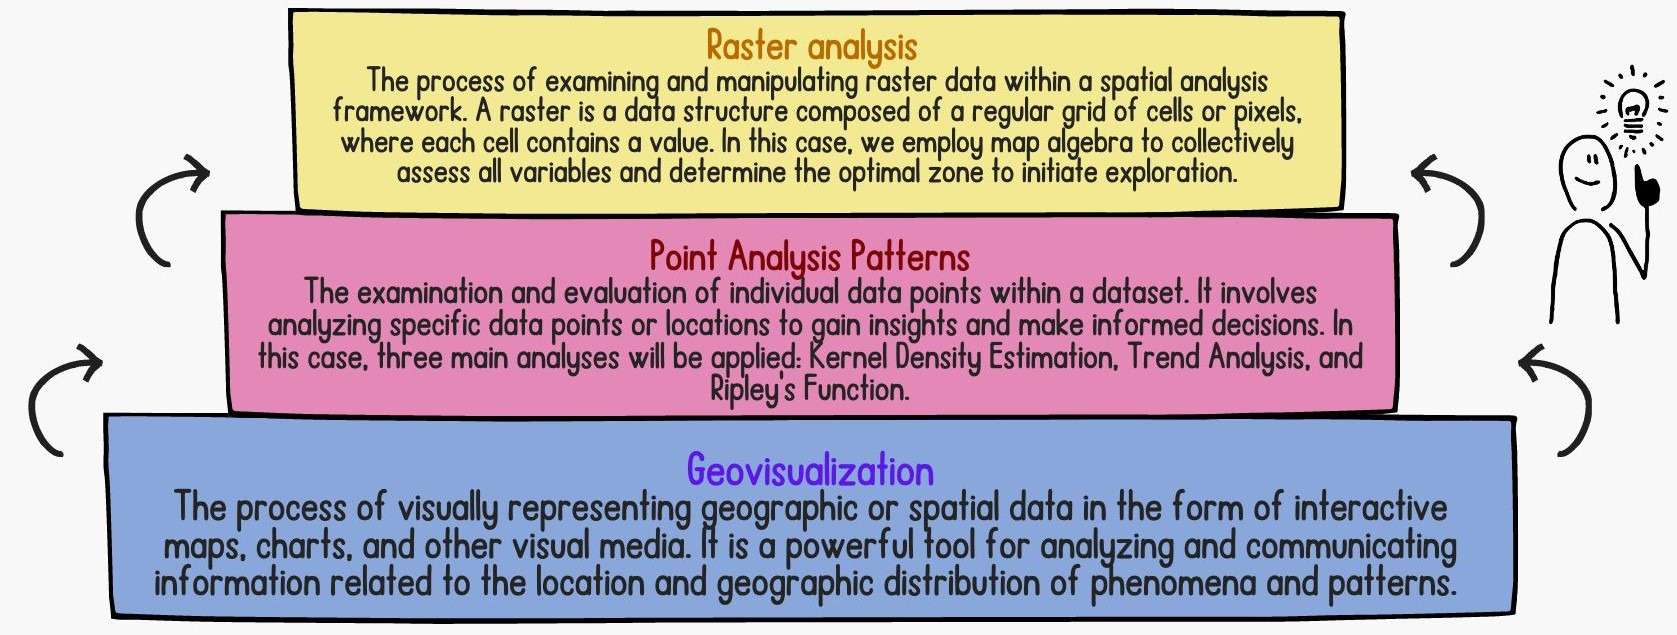
\includegraphics[width=1\linewidth]{img/metodologia}
	\caption[methodology]{Block diagram of the methodology applied in the study.}
	\label{fig:metodologia}
\end{figure}

Kernel Density Estimation: Kernel Density Estimation (KDE) is a statistical technique used to estimate the probability density function of a set of data points in a given area. It is commonly used in spatial analysis to identify areas of high or low density. This analysis can help identify hotspots, clusters, or areas of concentration within a dataset.

Trend Analysis: Trend analysis is used to identify and analyze patterns or trends in data over time. It involves examining the historical values of a variable to determine if there is a consistent upward, downward, or stable trend.

Ripley's Function: Ripley's Function, also known as Ripley's K-function, is a spatial statistical analysis tool used to examine the spatial pattern or clustering of data points. It measures the deviation of the observed spatial distribution of points from a random distribution. By comparing the observed distribution to a random distribution, Ripley's Function can identify clustering, dispersion, or regularity in the spatial arrangement of data points. 

\section{Results}
\subsection{CO2 emissions emitted by each city}
A geovisualization of CO2 emissions data by city was performed in the Sinu San Jacinto basin (Figure 2). Six cities were observed to produce a significant amount of CO2, with María La Baja, Cartagena, and El Carmen de Bolivar generating 1869.520 Kton/year as major contributors, and Barranquilla, Malambo, and Soledad producing 4171.81 Kton/year as the highest emitters.

\begin{figure}[h]
	\centering
	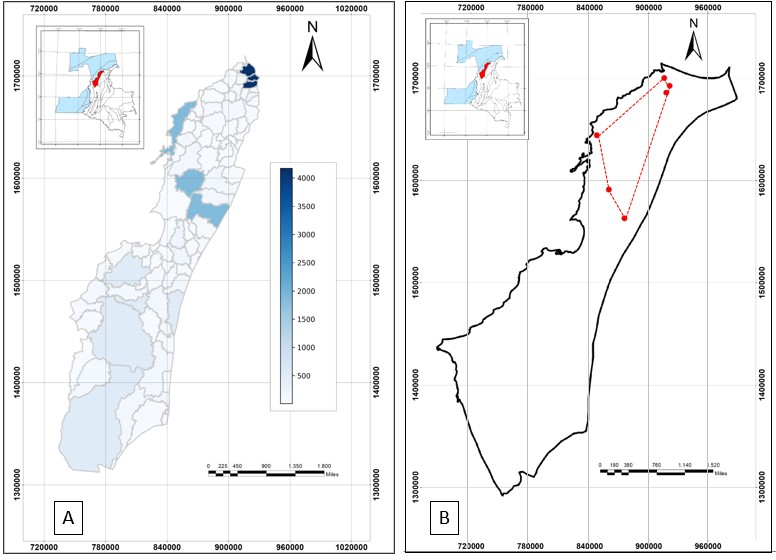
\includegraphics[width=1\linewidth]{img/Emisiones}
	\caption[Emisiones]{(A) Geovisualization of emissions emitted by each city located within the Sinu San Jacinto basin. (B) Zone between the centroids of the cities that produce the highest CO2 emissions.}
	\label{fig:emisiones}
\end{figure}
Alongside the geovisualization, an analysis of the centroids of cities with significant CO2 emissions was conducted to identify the closest zone among these cities (Figure 2).
\subsection{ANH Data}
In the analysis of point patterns, Kernel Density Estimation and Trend Analysis were applied to the available well data. Three data clusters were identified, with the northernmost cluster exhibiting a higher density of data compared to the other two clusters (Figure 3).
\begin{figure}[h]
	\centering
	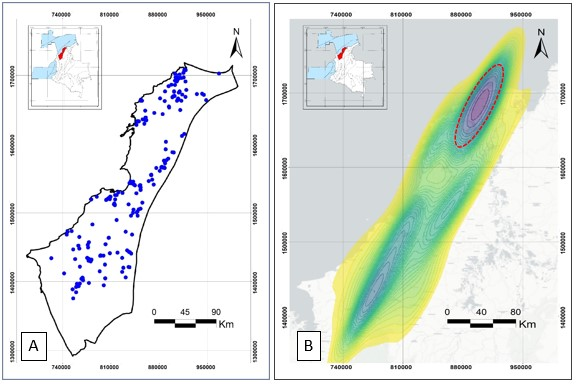
\includegraphics[width=1\linewidth]{img/Pozos}
	\caption{(A)Location of available wells in the ANH, located within the Sinu San Jacinto basin. (B)Kernel Density Estimation of the available wells by the ANH.}
	\label{fig:pozos}
\end{figure}


The 2D seismic lines data was transformed into a point shapefile, with points spaced every 5,000m along each line. The result of Kernel Density Estimation for these points reveals two concentrations of data density, one in the north and another in the south(Figure 4).
\begin{figure}[h]
	\centering
	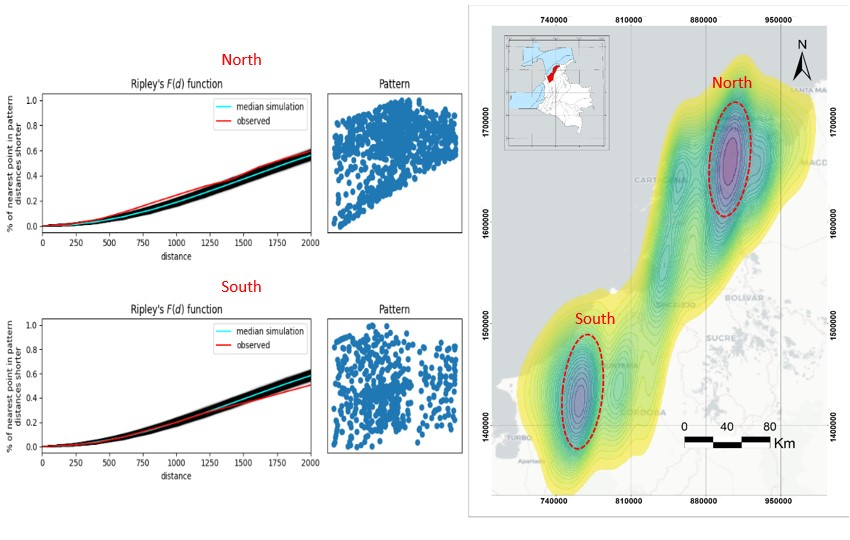
\includegraphics[width=0.8\linewidth]{img/sismica2d}
	\caption{Kernel Density Estimation and Ripley's Function analysis for the 2D seismic data.}
	\label{fig:sismica2d}
\end{figure}
Due to these two concentrations, the Ripley's Function is applied to compare the distances between the points. It is observed that the data distribution in the northern zone is more clustered than the data distribution in the southern zone(Figure 4).








\subsection{Seismicity}
Colombia is located within one of the most active seismic zones on Earth, as the Nazca and Caribbean tectonic plates converge against the South American plate in the region. Currently, the Servicio Geologico de Colombia has a map that classifies seismicity in Colombia into low (green), intermediate (yellow), and high (red) categories(Figure 5).

\begin{figure}[h]
	\centering
	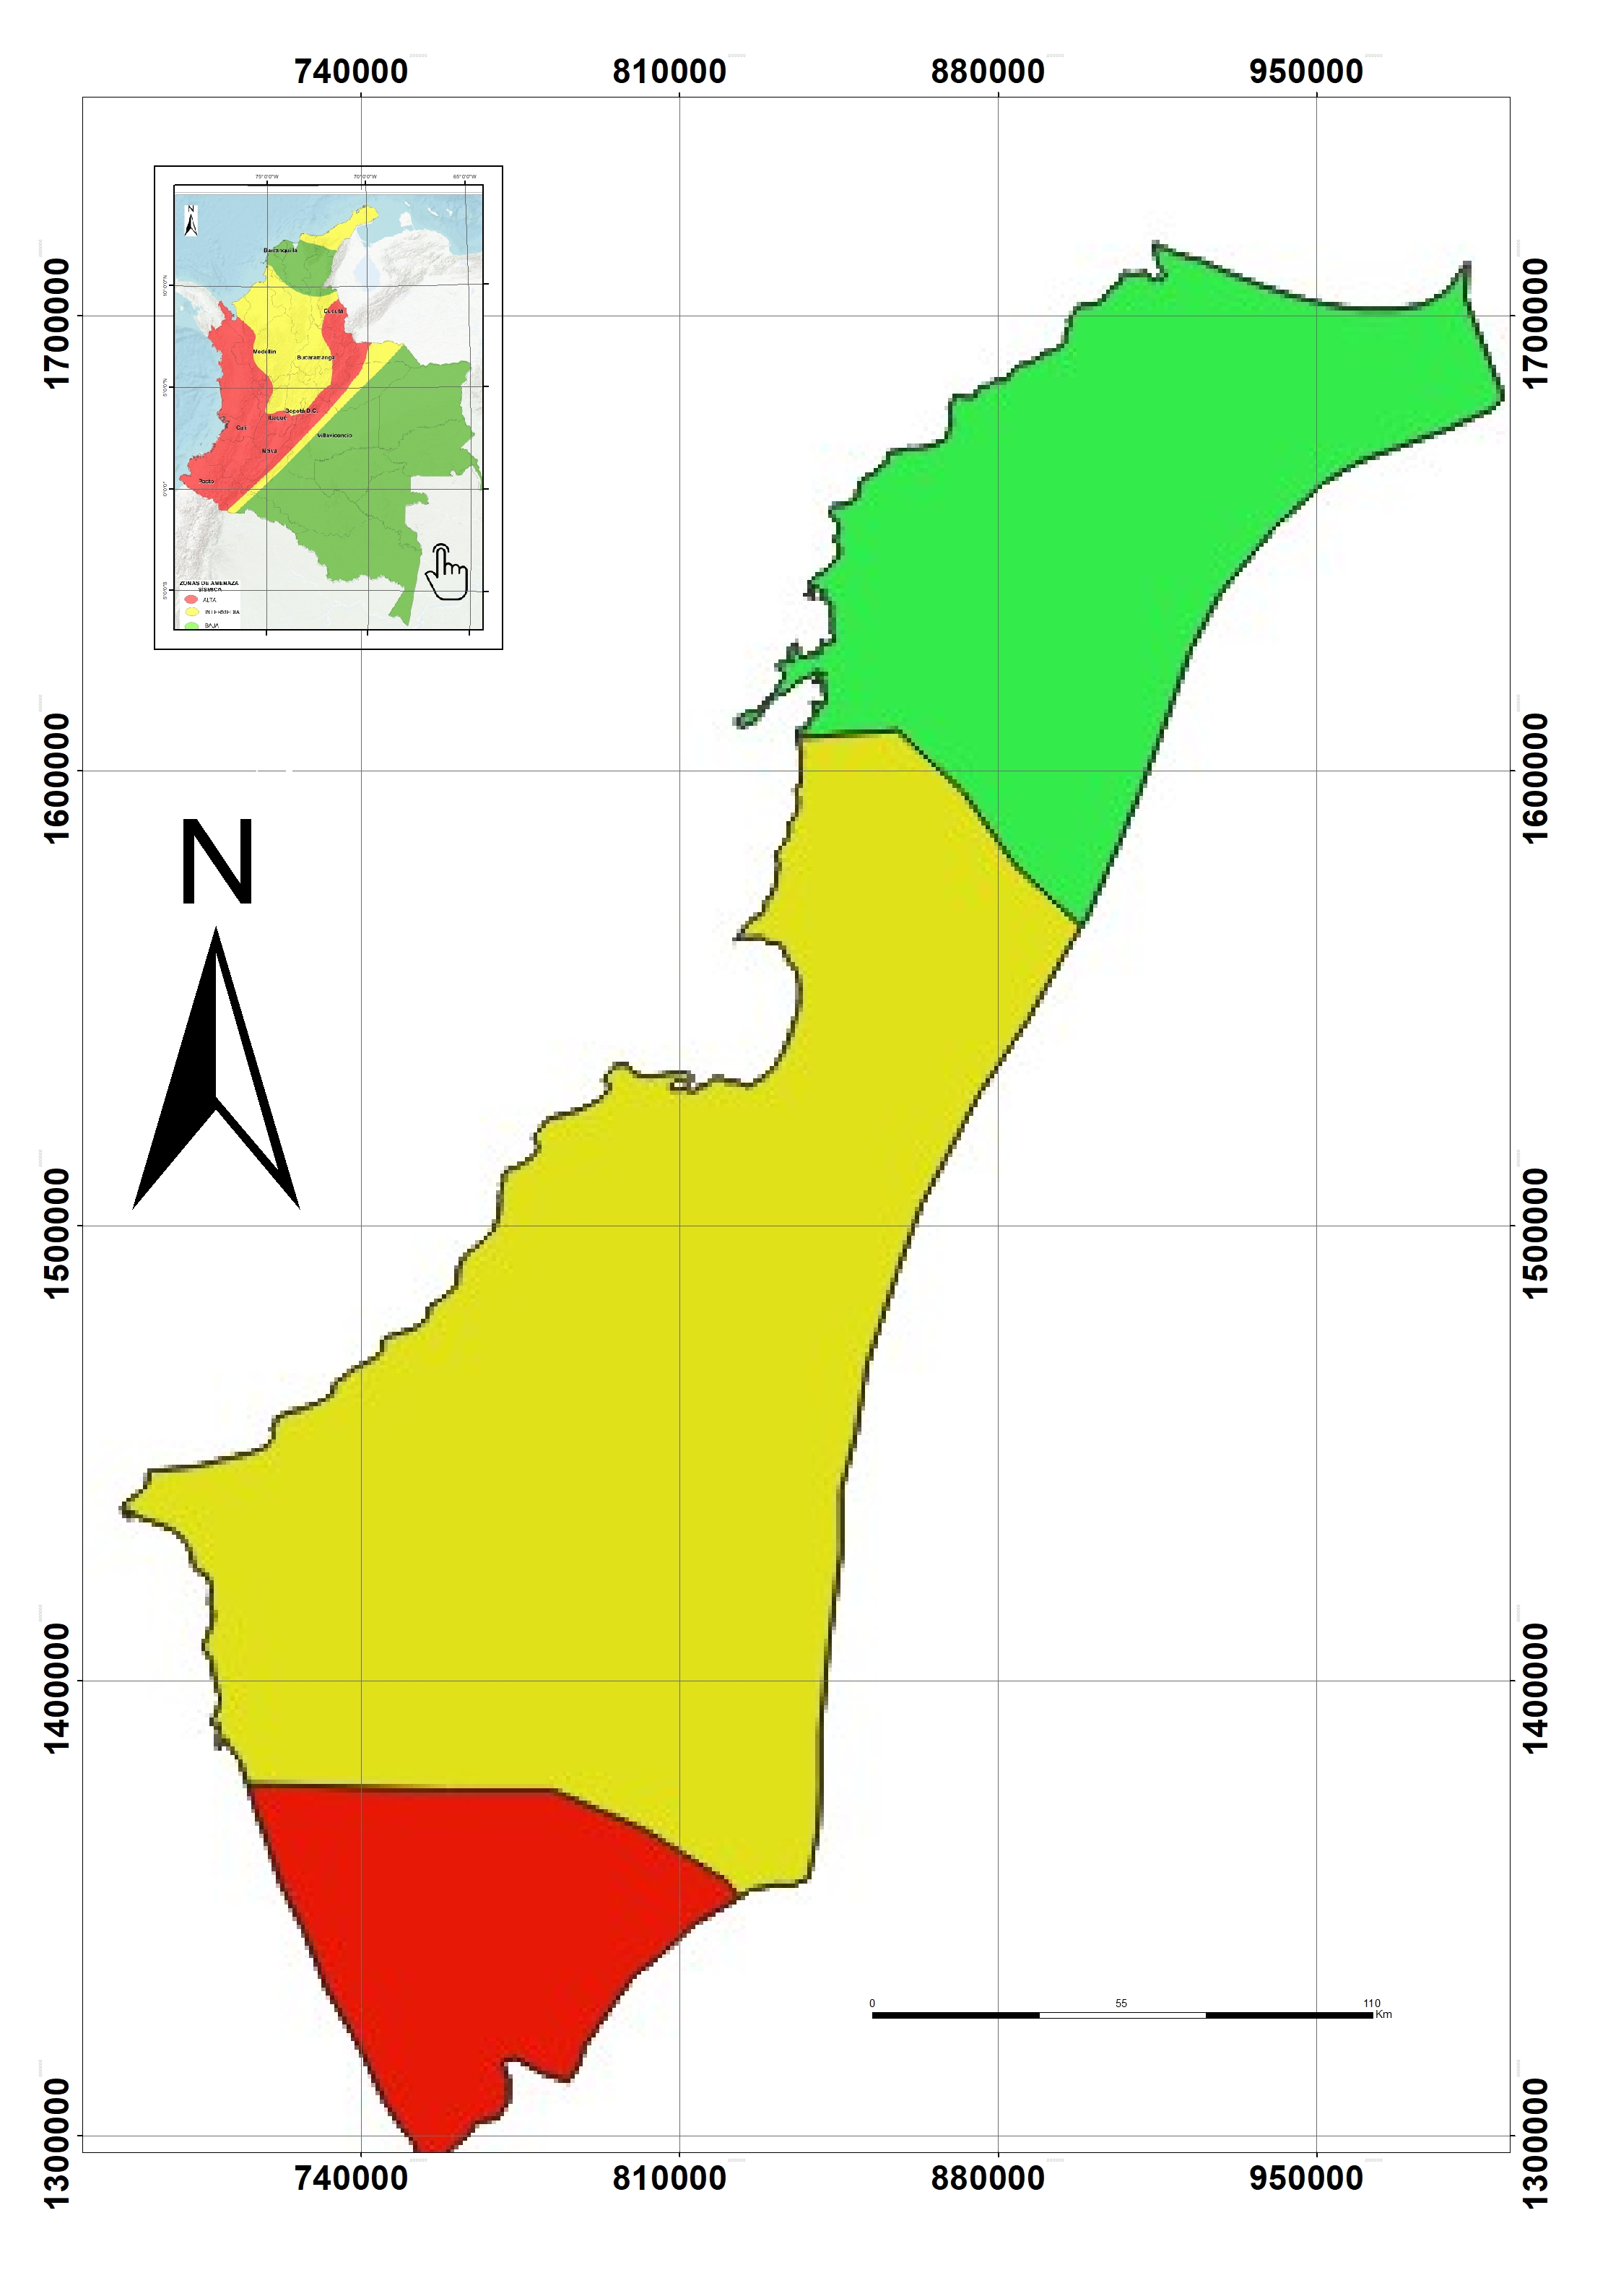
\includegraphics[width=0.5\linewidth]{img/Mapadesismicidad}
	\caption[Seismicity]{Map of seismicity in the Sinu San Jacinto basin. Taken and modified from the Geoportal of the Geological Service}
	\label{fig:mapadesismicidad}
\end{figure}
The zone with the highest seismicity in the Sinu San Jacinto basin is located in the southern part of the basin, near the subduction zone with the Nazca plate.

\subsection{Mud bodies}
A Kernel Density Estimation analysis is performed on the data of outcropping mud body locations(Figure 6), revealing a westward trend within the basin, corresponding to the location of the Sinu Onshore sub-basin, thus relating to the genesis of this sub-basin \cite{Rossello2022}.

\begin{figure}[h]
	\centering
	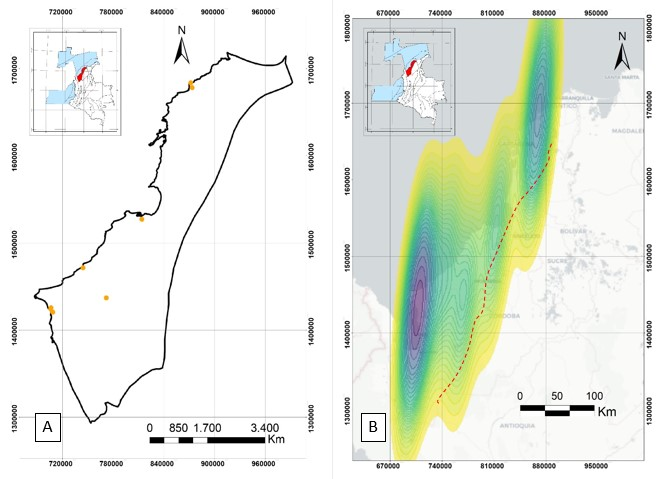
\includegraphics[width=0.8\linewidth]{img/Volcanesdelodo}
	\caption[Volcanes]{(A) Distribution of mud bodies in the Sinu San Jacinto basin. (B) Division of the Sinu San Jacinto basin into the Sinu Sub-basin to the west of the red line and the San Jacinto Sub-basin to the east of the red line.}
	\label{fig:volcanesdelodo}
\end{figure}

\section{Discussion}
Each of the variables analyzed previously plays a distinct role in the assessment of selecting the optimal area to initiate the exploration of underground CO2 storage zones. However, seismicity and the presence of mud bodies play a significant role in both the technical and environmental aspects of the project. Meanwhile, the proximity to major CO2 emission sources and data availability are factors that influence the economic viability of the project.

\subsection{Value of the variables}
The reclassification was carried out by assigning values from 1 to 5 to each variable, except for the Sinu Onshore sub-basin where a value of 0 was assigned due to the presence of mud bodies. This reclassification will enable a better representation of specific basin characteristics and facilitate subsequent processing using raster algebra.

\begin{figure}[h]
	\centering
	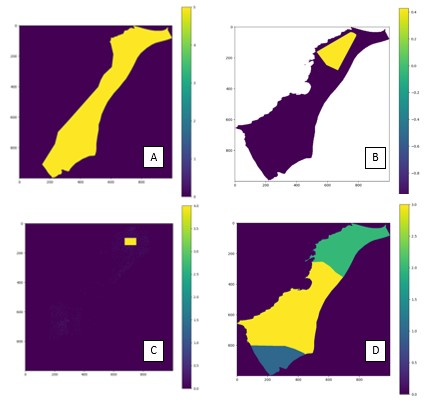
\includegraphics[width=0.7\linewidth]{img/Raster}
	\caption{ (A)sub-basin genesis classification. (B) Area enclosed the cities with the highest CO2. (C)Density of wells, 2D seismic, and 3D seismic. (D)Seismic activity.}
	\label{fig:raster}
\end{figure}

\subsection{The best area for underground CO2 storage exploration}
As a final result, a raster map of the optimal area for initiating underground CO2 exploration was obtained. This area is geologically located in the Luruaco Block. It is characterized by the presence of the Luruaco anticline as its main structure, which exhibits a more recent stratigraphic sequence compared to the San Jacinto and San Jerónimo sectors to the south (Figure 8).
\begin{figure}[h]
	\centering
	\includegraphics[width=0.7\linewidth]{img/Mapaáreadeinteres}
	\caption{Final result of map algebra.}
	\label{fig:mapaareadeinteres}
\end{figure}


\section{Conclusion}
1. Within the Sinu San Jacinto basin, the Luruaco Block is located in an area classified as low seismic risk by the SGC (Colombian Geological Survey). It is situated in a zone where no mud bodies are found, thus avoiding risks of CO2 escape. Moreover, it is an economically viable area for underground exploration and storage of CO2.

2. No zone within the Sinu Onshore sub-basin is recommended for underground CO2 storage studies.

3.The cities with the highest sources of CO2 emissions in the Sinu San Jacinto basin are associated with areas of manufacturing industries, oil and gas activities, and mining and quarrying sectors.

\section{Recommendations}
It is recommended to conduct more recent studies on CO2 emissions measurement for future studies of prospecting storage zones. Similarly, the investment in acquiring 3D seismic data is recommended, as it is crucial for this type of study.


\bibliography{ifacconf}             % bib file to produce the bibliography
                                                     % with bibtex (preferred)
                                                   
%\begin{thebibliography}{xx}  % you can also add the bibliography by hand

%\bibitem[Able(1956)]{Abl:56}
%B.C. Able.
%\newblock Nucleic acid content of microscope.
%\newblock \emph{Nature}, 135:\penalty0 7--9, 1956.

%\bibitem[Able et~al.(1954)Able, Tagg, and Rush]{AbTaRu:54}
%B.C. Able, R.A. Tagg, and M.~Rush.
%\newblock Enzyme-catalyzed cellular transanimations.
%\newblock In A.F. Round, editor, \emph{Advances in Enzymology}, volume~2, pages
%  125--247. Academic Press, New York, 3rd edition, 1954.

%\bibitem[Keohane(1958)]{Keo:58}
%R.~Keohane.
%\newblock \emph{Power and Interdependence: World Politics in Transitions}.
%\newblock Little, Brown \& Co., Boston, 1958.

%\bibitem[Powers(1985)]{Pow:85}
%T.~Powers.
%\newblock Is there a way out?
%\newblock \emph{Harpers}, pages 35--47, June 1985.

%\bibitem[Soukhanov(1992)]{Heritage:92}
%A.~H. Soukhanov, editor.
%\newblock \emph{{The American Heritage. Dictionary of the American Language}}.
%\newblock Houghton Mifflin Company, 1992.

%\end{thebibliography}
                     
\end{document}
